\subsubsection{Modeling Withdrawals, Discharges and Consumptive Use}
\label{sec:consumptive-use}


\begin{multicols}{2}
% Commented as this echos something from conclusions
% Total water withdrawal demand in Virginia is expected to increase from approximately 6,000 MGD in 2020, to over 7,000 MGD in 2040, with the majority of this total demand used for power generation. Non-power generation related withdrawals are projected to grow from nearly 1,600 MGD in 2020 to nearly 1,900 MGD in 2040.  
\noindent While the majority of surface water withdrawals are returned to streams and estuaries as point source discharges, a significant fraction leaves the system as irrigation, evaporation/transpiration, transmission losses, finished products from manufacturing, or human and livestock consumption. As previously mentioned, the portion of water that is not returned to the system is referred to as ``Consumptive Use" (CU). This is an important variable in calculating a current and future water balance, therefore its application in a model warrants consideration. \medskip

\noindent The amount of consumption in Virginia ranges from between 1\% to 100\% depending on the use type and season.  Summer CU is nearly twice that of CU in the winter (see Figure \ref{fig:cumonthly}).  Municipal withdrawals amount to approximately 60\% of all non-power withdrawals in 2020 and are therefore responsible for much of the monthly variation and future growth in CU shown in Figure \ref{fig:cumonthly}. Statewide monthly CU for all non-power uses is estimated as varying from between 200 to 400 MGD in 2020.  Non-power uses are isolated in order to highlight the monthly trends in non-power facilities, as power facilities are generally considered non-consumptive. The peak monthly CU for non-power facilities is estimated to be nearly 500 MGD by 2040.  
\end{multicols}




% Note: to refer to figure in document by using
% the "\ref" tag, like: \ref{fig:cumonthly}
% use of {figure} block with associated
% "\label", and "\caption" are both needed to 
\begin{figure}[h]
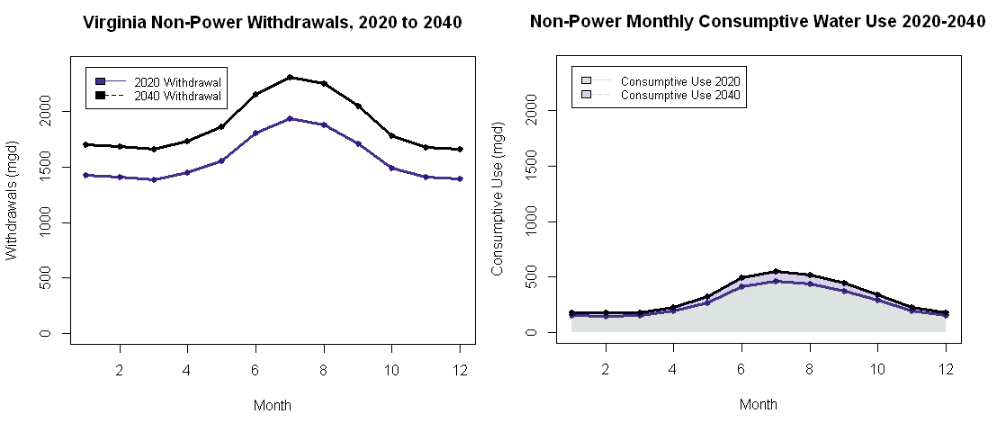
\includegraphics[scale=1.0]{sections/Xfigures/cu_monthly_2020-2040_2-panel.png}
\caption{Average monthly simulated withdrawals (left) and consumptive use (right) for all uses except power generation.  Simulated values for 2020 are based on a total annual demand of nearly 1,600 MGY, and 2040 are based on an annual demand of approximately 1,900 MGY.}
\label{fig:cumonthly}
\end{figure}

\paragraph{Estimating Consumptive Use Factors}\mbox{}\smallskip

\begin{multicols}{2}
\noindent Throughout 2017-2019 DEQ collaborated with the Virginia Tech Department of Biological Systems Engineering through a USGS Water-Use Data and Research program (WUDR) grant on a project titled “Virginia’s Consumptive Use Data Transfer, Export, and Analysis.”\footnote{McCarthy (2019), \href{http://hdl.handle.net/10919/89928}{http://hdl.handle.net/10919/89928}} Primary results of this project include the development of a set of data retrieval tools to supply point source NPDES Discharge Monitoring Report (DMR) data to Virginia’s VAHydro data system. By applying the tools developed through this project, DEQ was able to incorporate all reported point source discharges from Virginia and surrounding states into VAHydro.\medskip 

\noindent Using this wealth of historic discharge data, CU factors (representing the fraction of a withdrawal that is considered consumptive) can be developed. CU 
\end{multicols}

\pagebreak

\newgeometry{left=1in,right=1in,bottom=1in,top=1in}

~\par\vspace{-\baselineskip} %required for a wrapfigure right after section

\begin{wrapfigure}{r}{0.50\linewidth}
    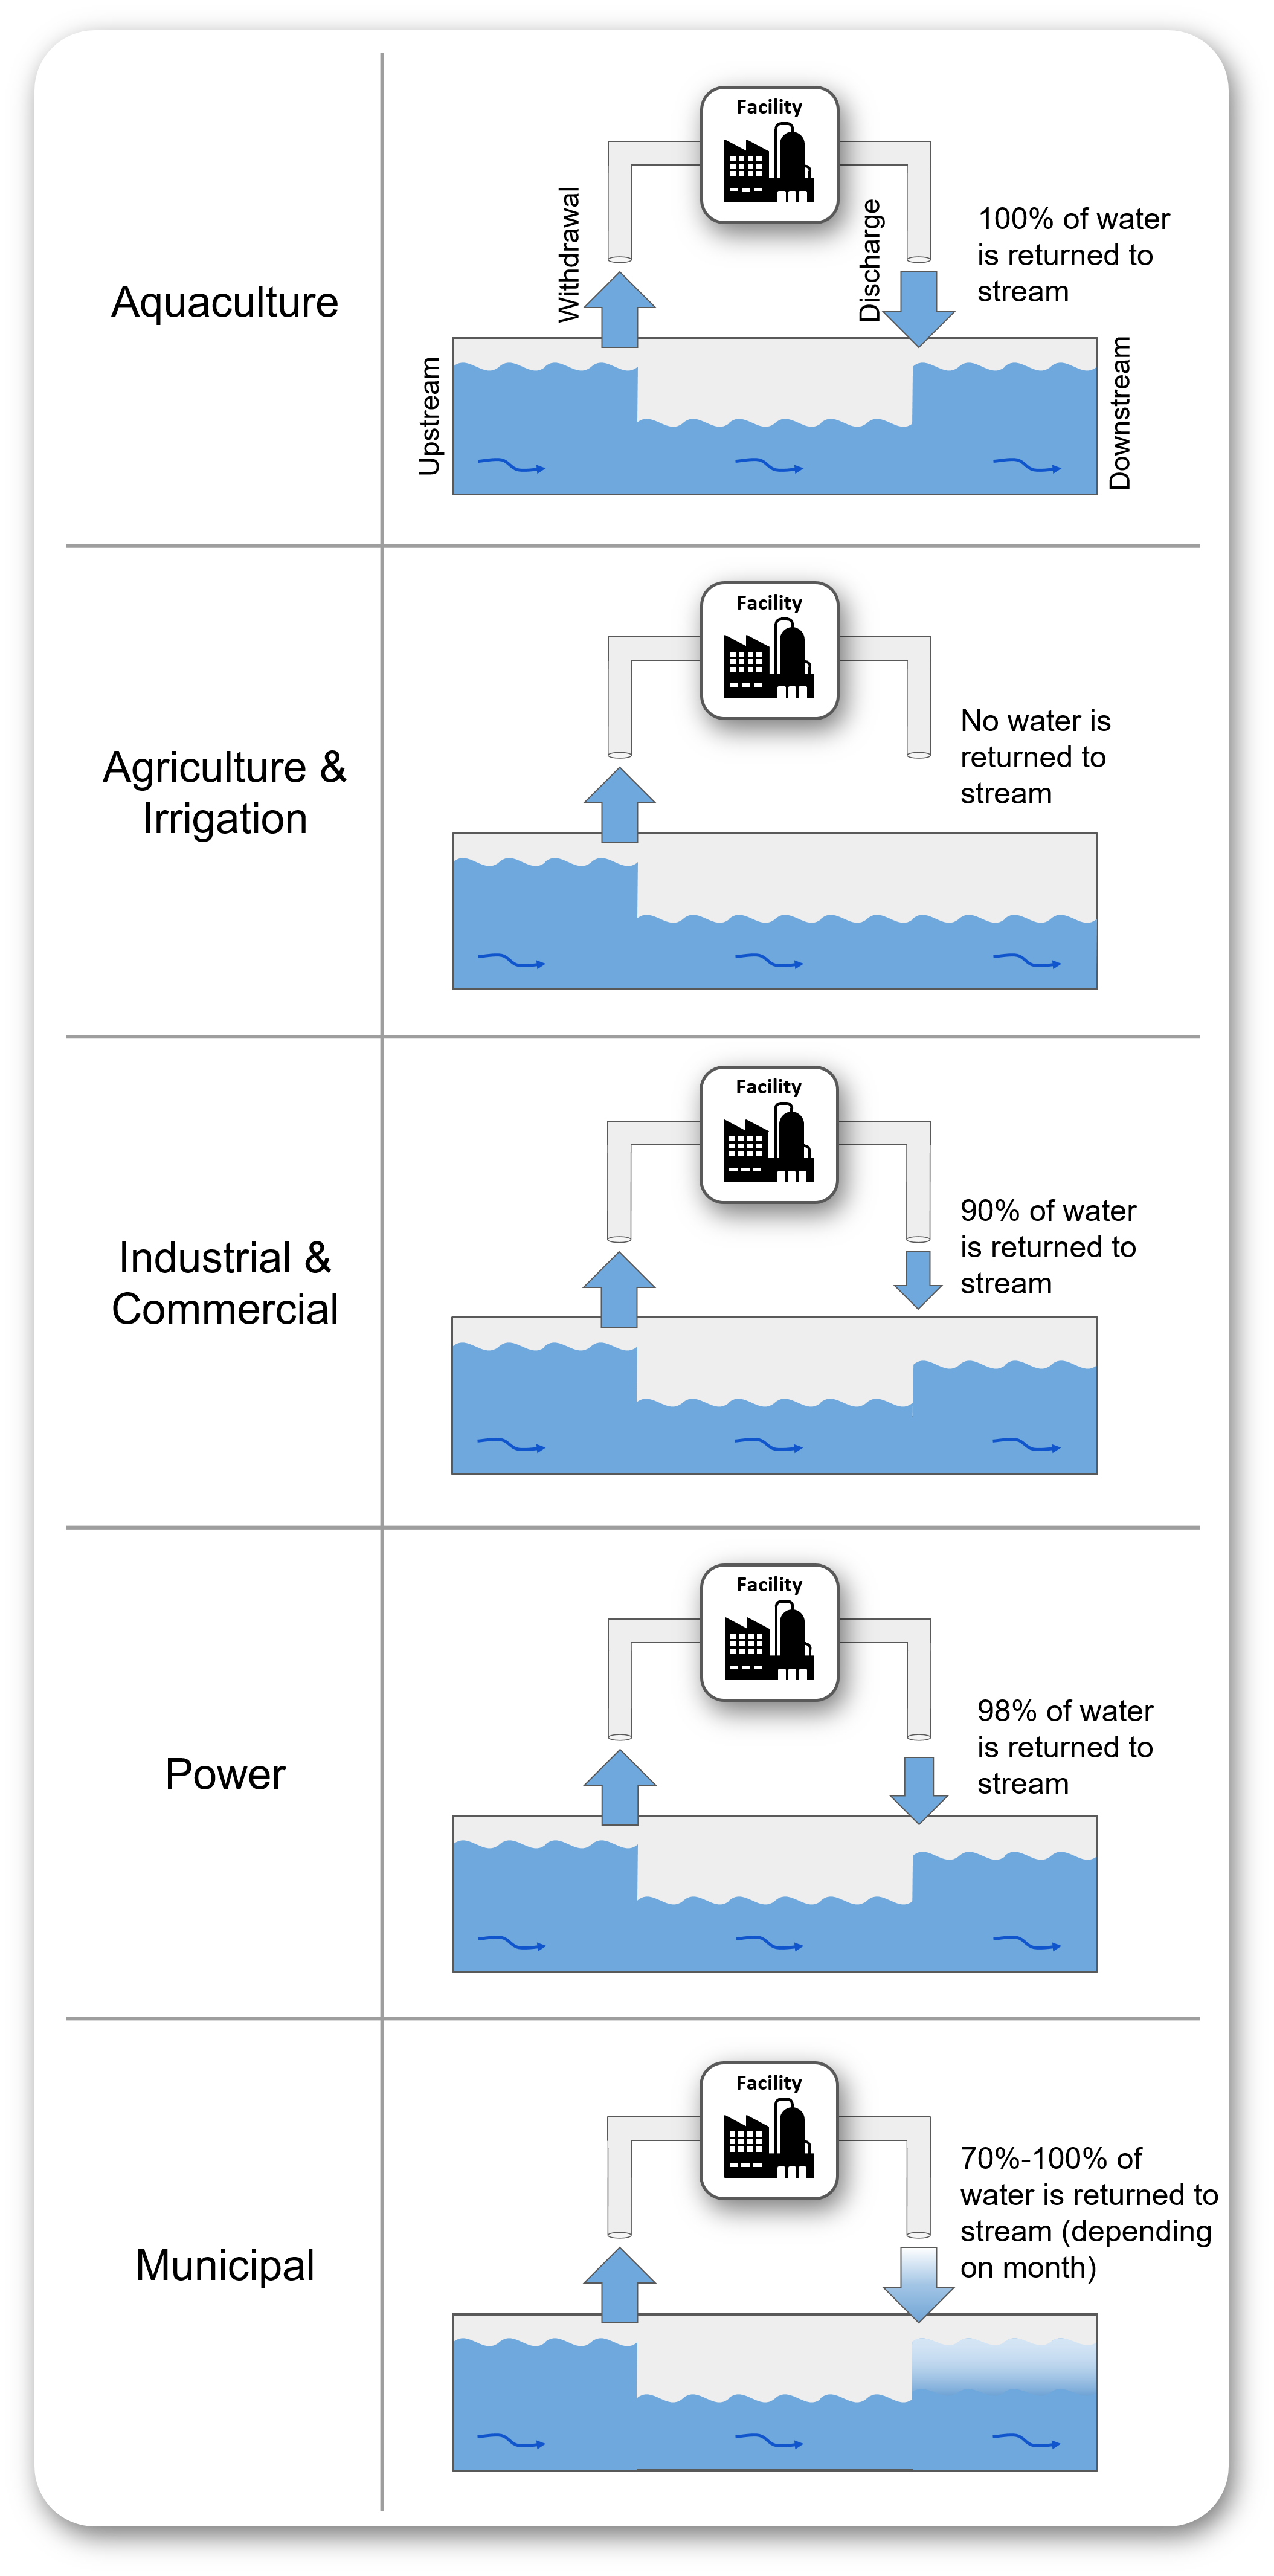
\includegraphics[width=0.60\textwidth]{sections/Xfigures/CU_SectorFactor_Graphic.png}
    \caption{\small Impact of sector-level consumptive use factors on a stream system where the discharge point is located downstream of the intake. Also depicted is the reduction in streamflow that can occur between the intake and the discharge for systems that are not fully consumptive.}
    \label{fig:CU_SectorFactor_Graphic.png}
\end{wrapfigure}

\noindent factors are a critical component of the VAHydro model, and a necessary prerequisite for modeling future scenarios. By multiplying water demands (such as facility-level 2020 or 2040 demand) by a CU factor, the model is able to scale those demands to more accurately simulate the overall water balance of the stream system.\bigskip  

\noindent These percentages are calculated using several methods depending on data availability and use type.  When reliable long-term withdrawal and discharge data is known for a given system, CU factors specific to that system are used.  Most municipal systems are estimated by using the ``winter base rate" method, provided that long term monthly withdrawal data is available.  This method estimates summer time CU as the difference between summer and winter time demands (see \ref{sec:cu_wbr}). The remainder of systems were estimated based on analysis of NPDES data and comparison with CU values from scientific literature in the eastern United States.\footnote{McCarthy (2019), \href{http://hdl.handle.net/10919/89928}{http://hdl.handle.net/10919/89928}} Because return flows are calculated as a function of the amount of water withdrawn, the resulting models can better represent seasonal trends in CU, the effects of addition or removal of facilities, and the ability to project changing point source flows based on changes in future demands.  Table \ref{tab:Consumptive Use Factor Defaults} shows the default values for the various categories in this analysis.
%\end{multicols}
\bigskip

\vspace{-6mm}


%\begin{center}
\begin{table}[htp]

\caption{Consumptive Use Factor Defaults \hspace{250pt}}
\label{tab:Consumptive Use Factor Defaults}
%\begin{center}
\begin{tabular}{lllll}
\toprule
Sector Name & Factor Source                  & Factor \\
\midrule
\rowcolor{gray!6}  Aquaculture          & VPDES Matched                  & 0\% \\
Agriculture          & Literature median              & 100\%   \\
\rowcolor{gray!6} Irrigation           & Literature median              & 100\%     \\
Industrial           & Literature                     & 10\%    \\
\rowcolor{gray!6}  Commercial           & Literature             & 10\% \\
Power           & VPDES Median/            & 2\% \\
           & Literature            &  \\
\rowcolor{gray!6}  Municipal            & Winter Base Rate                     & 0-30\%   \\
\rowcolor{gray!6}              &                      & by month   \\
\bottomrule 
\end{tabular}
%\end{center}
\end{table}
%\end{center}



%\end{multicols}

\vspace{-2mm}
\paragraph{Modeling Consumptive Use}\mbox{}\smallskip
\label{sec:cu_modeling}

%\begin{multicols}{2}
\noindent The VAHydro model estimates the amount of water returned to the stream each day by subtracting the CU percent from the total daily withdrawal, then routing the return flow to the next downstream river segment unless an alternative return point is known. Because total annual, and monthly percent of annual demand is the same for each year for a given scenario, monthly CU does not vary from year 
\restoregeometry

\begin{multicols}{2}
\noindent to year within any given scenario. This may underestimate some increases in demand in dry years when drought restrictions are not in place, and overestimate CU during wetter years.  Future analyses should include variations in demand based on meteorological factors to assess drought flow reductions due to CU occurring early in drought periods before restrictions are in place.\bigskip

\noindent \textbf{Location of Withdrawals and Return Flows}\smallskip
\label{sec:cu_return_loc}

\noindent Most surface water withdrawn is used, treated and returned to the same river some miles downstream of the withdrawal.  When the location of a return flow is known, models are configured to route return flow to the model river segment of the outfall location.  When return flow locations are not known, return flows are modeled as returning to the stream in the next downstream watershed from the point of withdrawal (see Figure \ref{fig:cu_loc}). Some systems (especially large municipal service areas) are structured such that discharge points are located in entirely different watersheds from their withdrawal. For example, the withdrawals in Spotyslvania County's Ni River Reservoir are used in the northern portions of that reservoir, and the majority of treated wastewater flows are returned to the tidal section of the Rappahannock River.  DEQ's model is generally adjusted to simulate these effects where they are known to occur.\bigskip

% \begin{figure}[H]
% \centering
% 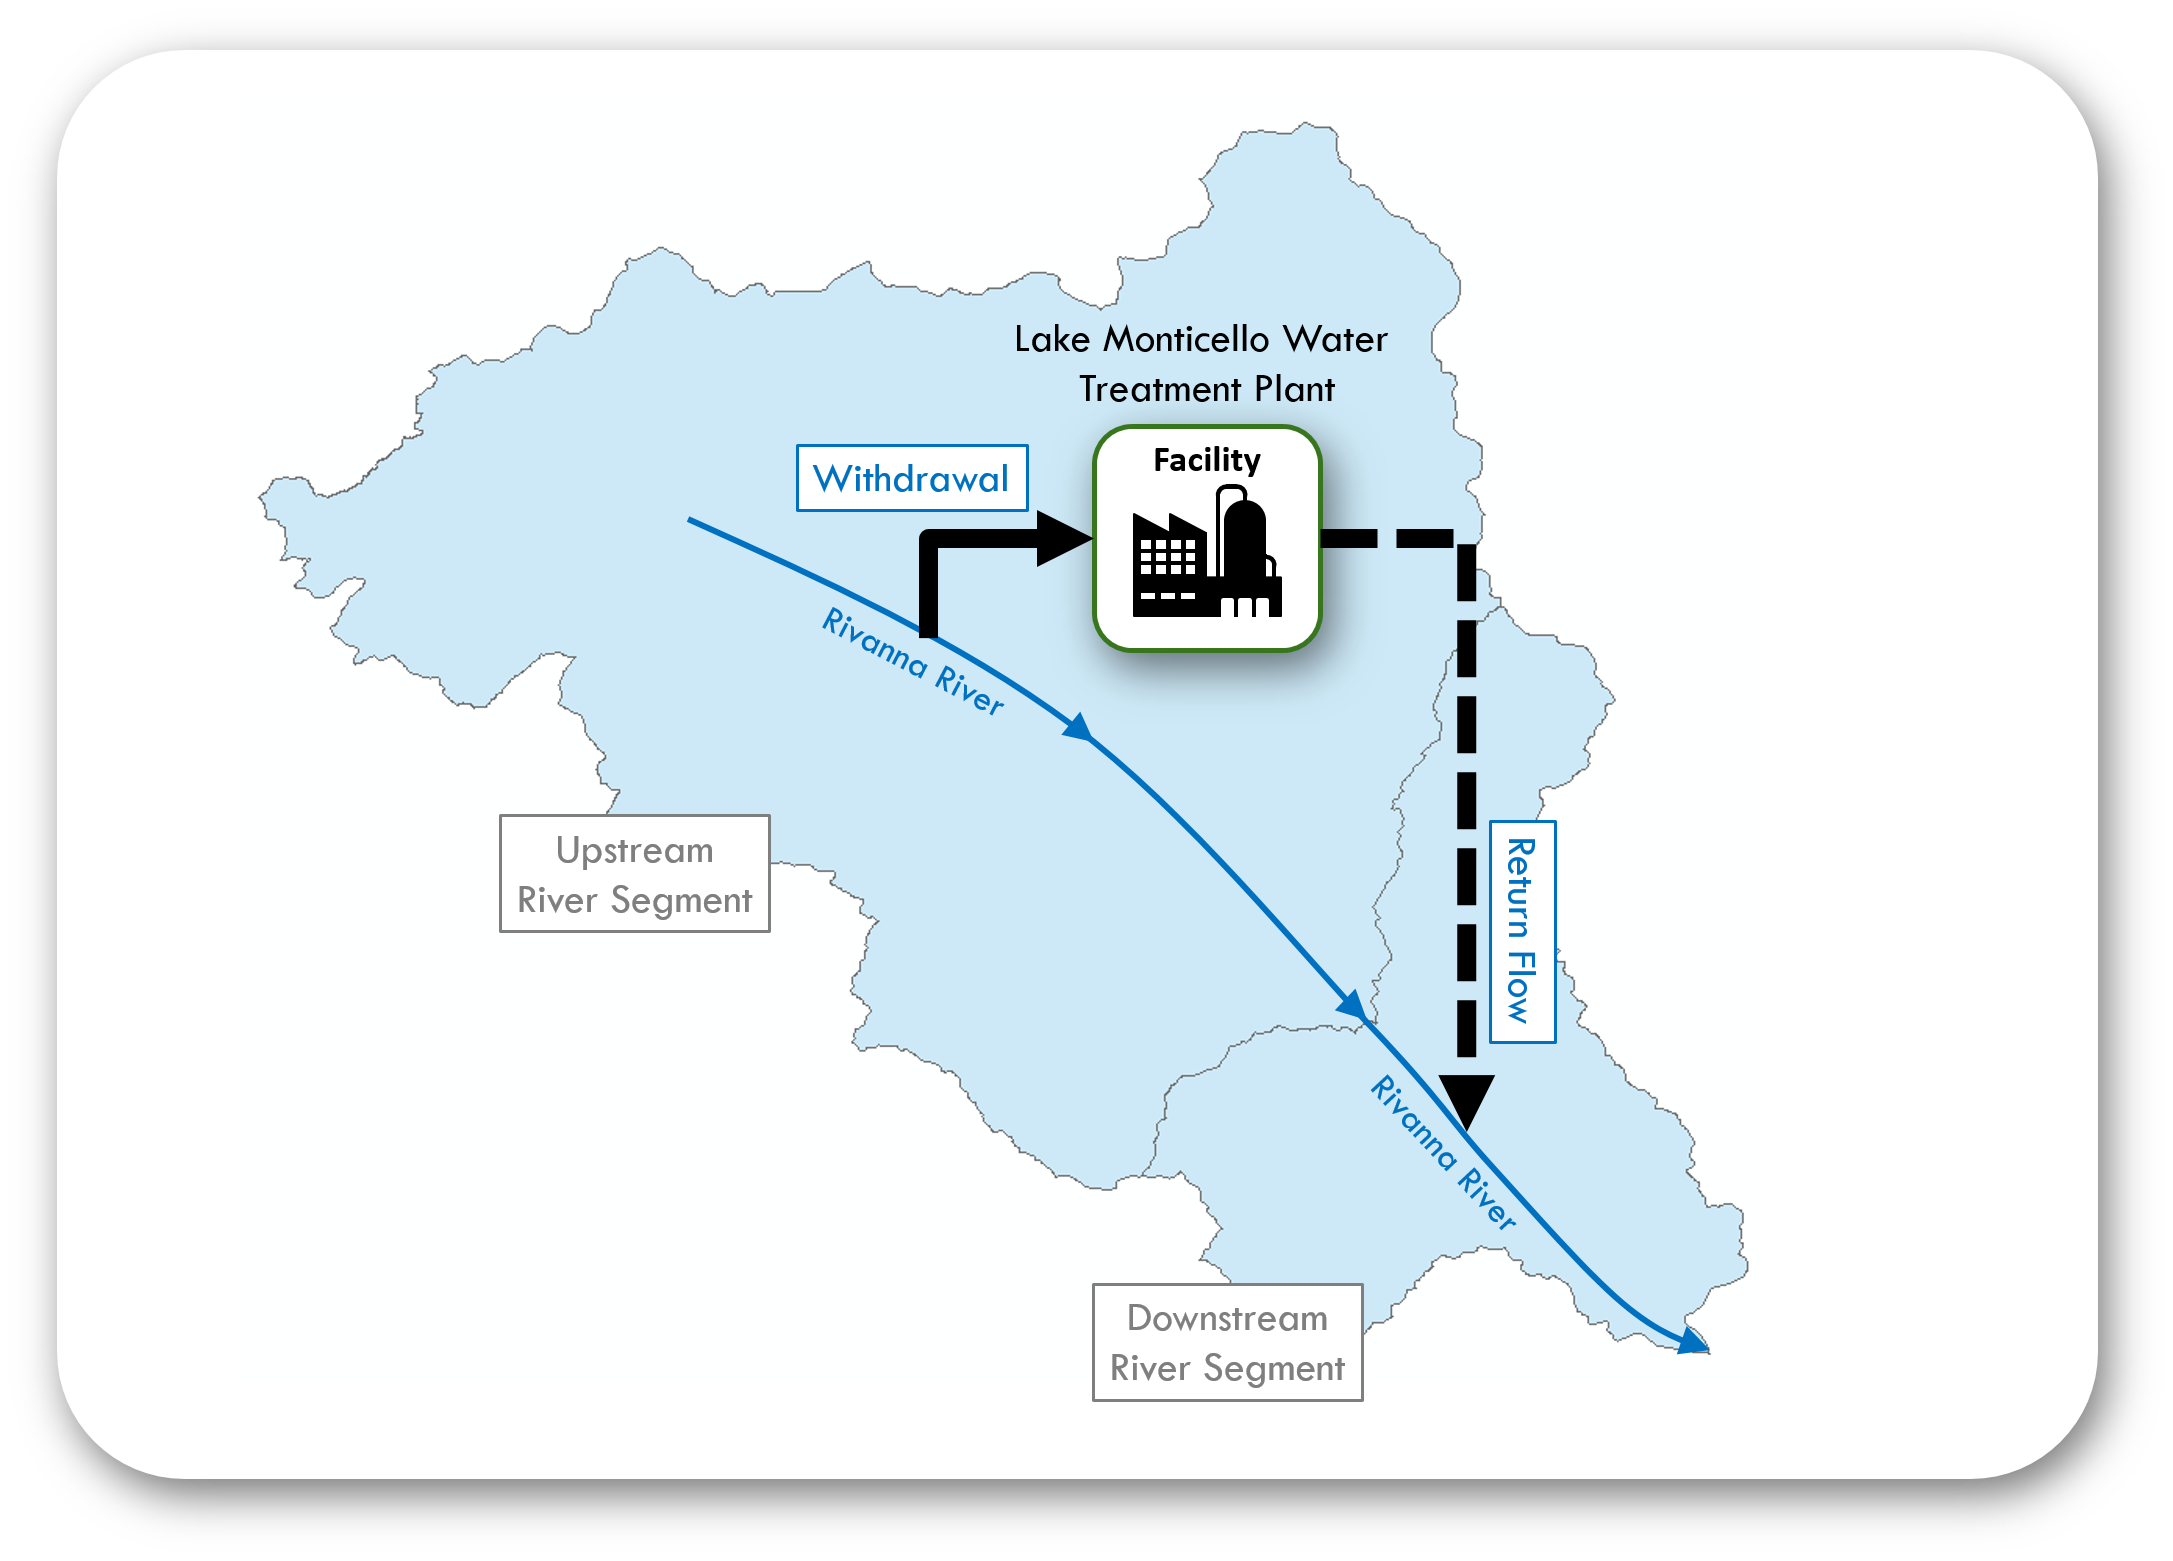
\includegraphics[width=5.1in]{sections/Xfigures/cu_return_flows.png}
% \caption{Default location of return flows from municipal wastewater treatment.}
% \label{fig:cu_loc}
% \end{figure}

\noindent \textbf{Low Flow Increases due to Withdrawals from Reservoirs and Groundwater}\smallskip
\label{sec:cu_lowflows}

\noindent In general, CU should result in a net decrease in stream flows, with a greater decrease during times of drought due to the smaller baseline water budget.  However, due to the use of ``stored water", namely reservoirs and groundwater pumping, some streams will actually see an increase in low flows. This is because instead of pumping directly from streams during drought, water is withdrawn from reservoirs or groundwater wells, then returned to streams as a result of the wastewater treatment process.  Not all groundwater pumping is assumed to be returned to the stream.  Groundwater withdrawals are only assumed to be returned to streams if they are a) part of a conjunctive system with surface water intakes, or b) part of a municipal system with total groundwater withdrawals $>$ 100 MG in a single year.  Domestic private well withdrawals (Small Self-Supplied Users) are assumed to be treated on-site (septic), and therefore do not add or subtract from the stream water balance.
\end{multicols}



%\newgeometry{bottom=1in,top=0.8in,left=1in,right=1in}

\begin{figure}[H]
\centering
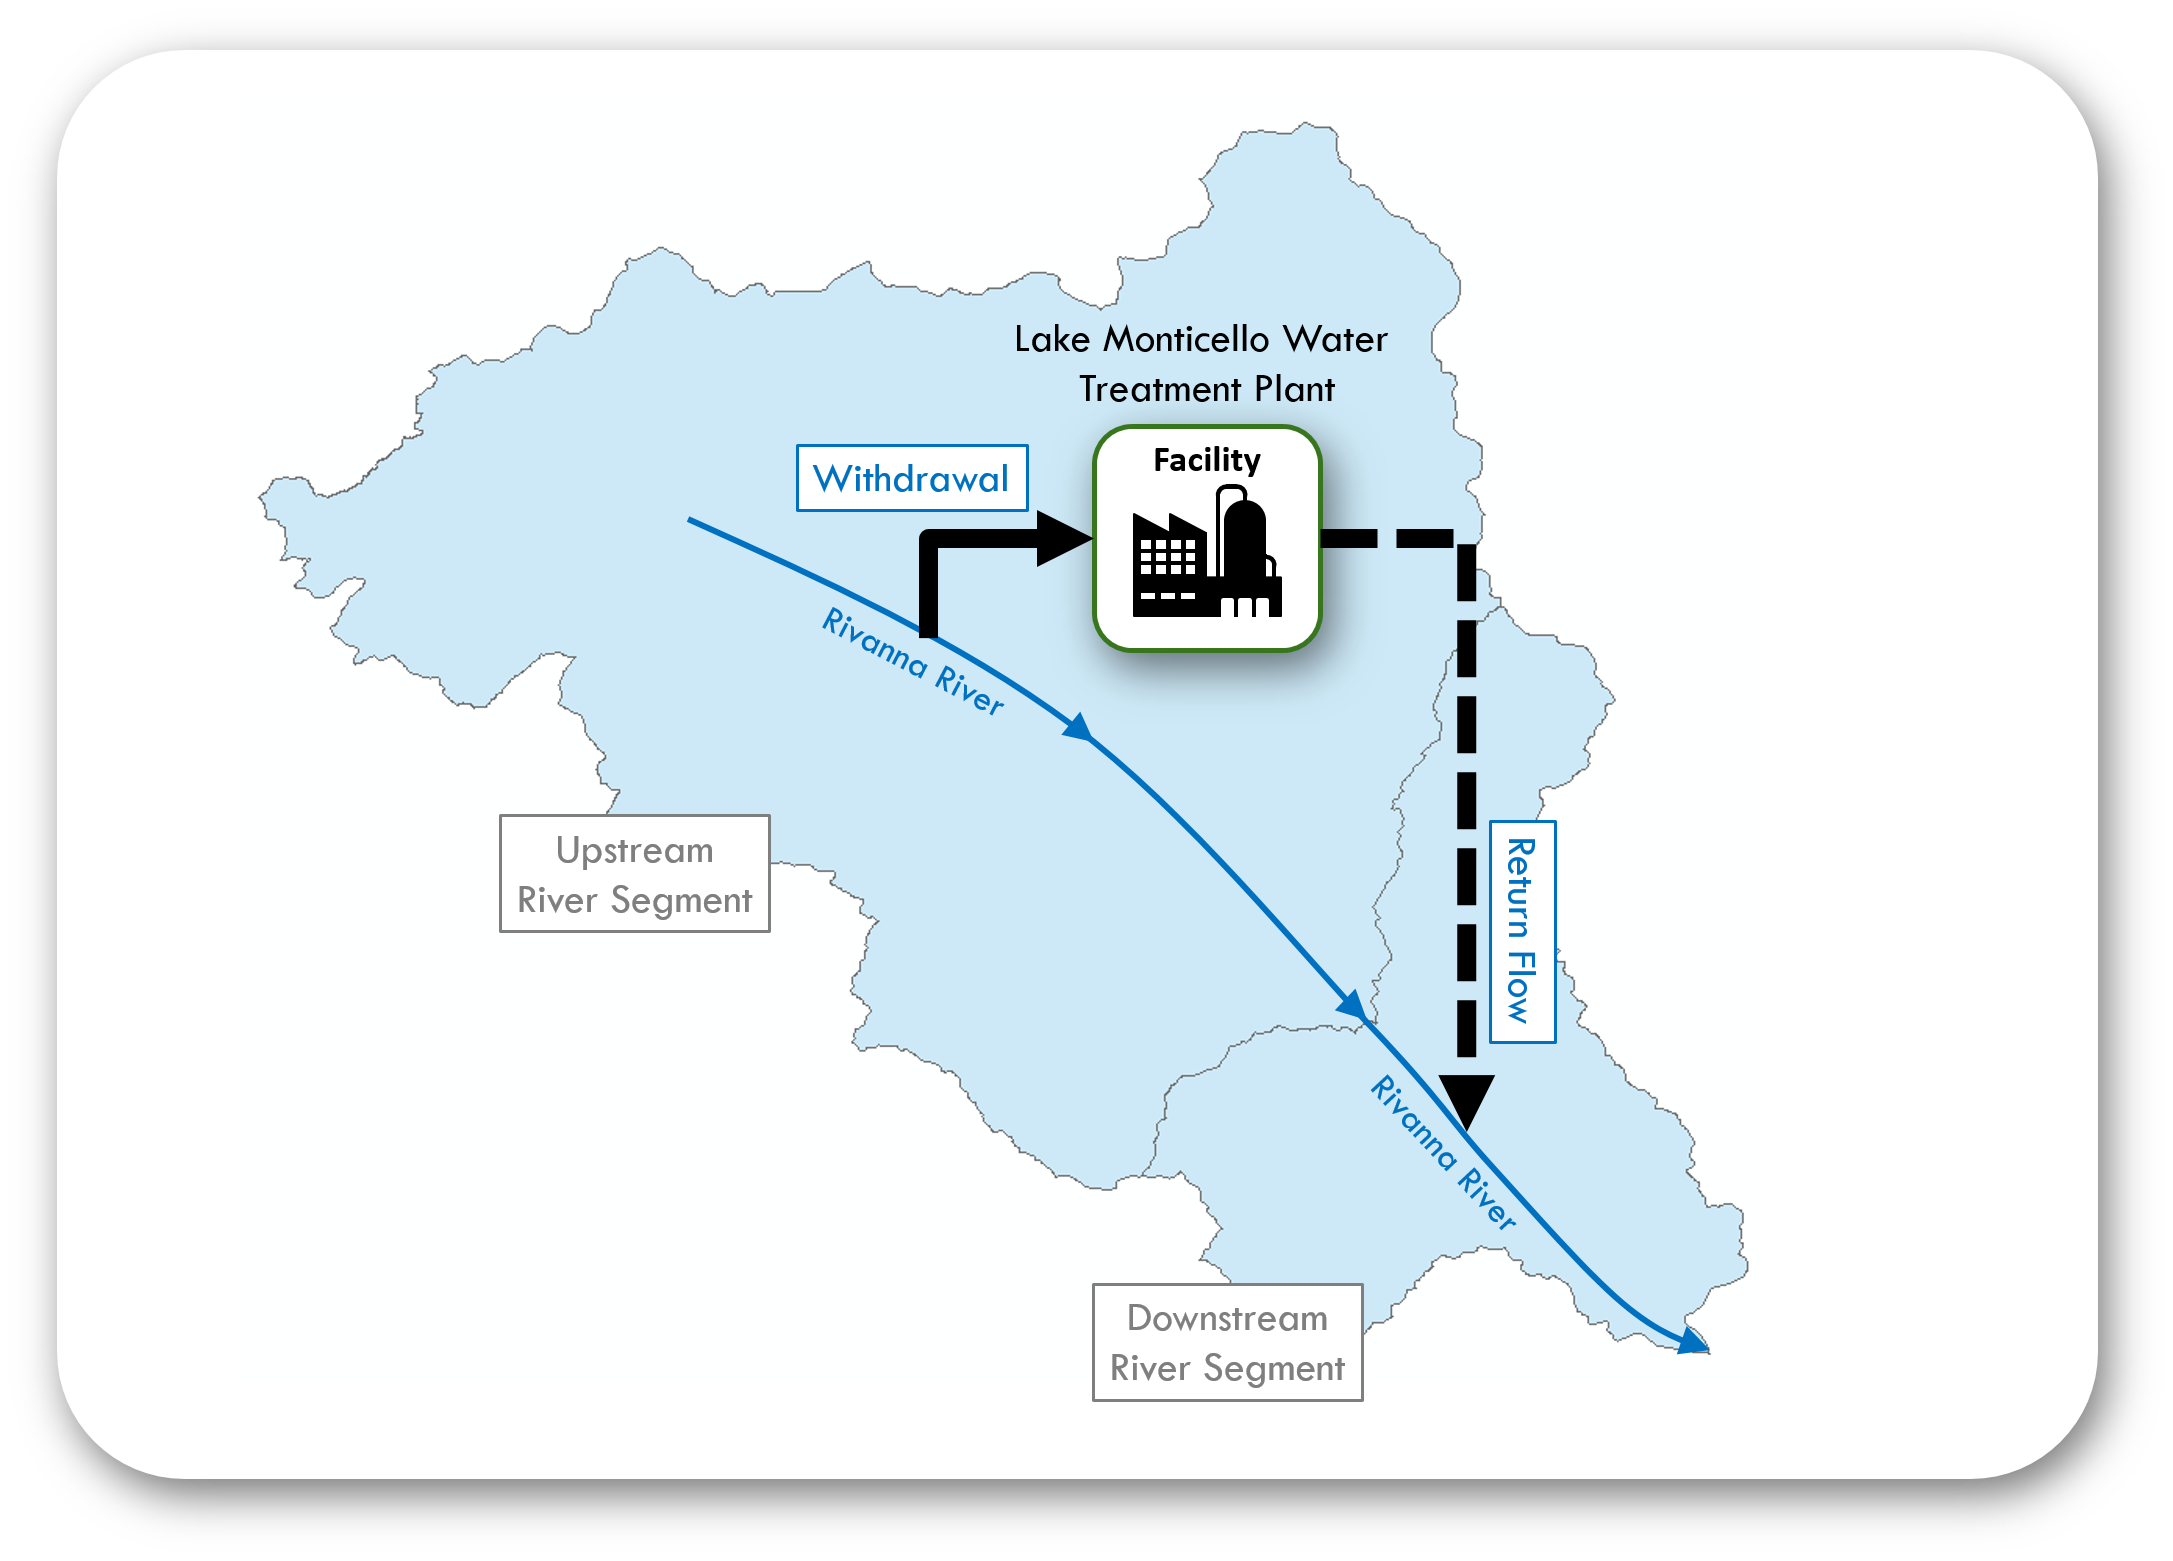
\includegraphics[width=5.1in]{sections/Xfigures/cu_return_flows.png}
\caption{Default location of return flows from municipal wastewater treatment.}
\label{fig:cu_loc}
\end{figure}

\begin{multicols}{2}


\noindent \textbf{Consumptive Use for Power Plant Cooling}\smallskip
\label{sec:cu_power}

\noindent Power plants without historical data are assumed to have a CU percentage of 2\%, based on the median value from the 2018 VPDES study. Despite a 2020 average daily demand of approximately 3,000 MGD (3 billion gallons per day) in Virginia's non-tidal rivers (including power plants in the WV and MD parts of the Potomac), evaporative losses from cooling amount to less than 100 MGD in total CU.\bigskip 

\noindent \textbf{Municipal Withdrawals Using Winter Base Rate Method}\medskip
\label{sec:cu_wbr}

\noindent Where possible, CU for public water supply withdrawals with long-term records are estimated using a variation on the ``winter base rate method" \cite{Ducnuigeen2015}; \cite{Li2017}, plus a standard factor for transmission losses (10\%, see \ref{sec:cu_tloss}). This method relies upon the assumption that outside watering activities are minimal during the winter, which is a valid assumption throughout Virginia. However, in some areas where winter demands are higher than summer, the WBR is not applicable. For those systems, we used the ``Standard Municipal Distribution" given below.  Figure \ref{fig:cu_wbr_summary} shows the range of consumptive use fractions/percentages, which are as low as 0.1 (10\%) during winter months, and as high as 0.4 (40\%) during summer months in a small subset of systems.  

\begin{itemize}
    \item ``Standard Municipal Distribution": CWS systems with seasonal populations or large industrial users are estimated with a standard municipal distribution, based on the ``winter base rate method" for Virginia as a whole. 
    \item \emph{In the Potomac River basin outside of Virginia} an analysis of CU was performed by ICPRB.  Demands in West Virginia, Maryland, and Pennsylvania were compiled by ICPRB, with CU factors that were obtained from a combination of site-specific (where available), and literature factors (see \cite{icprb2020}).
\end{itemize}

\end{multicols}
%\restoregeometry

\vspace{-6mm}
\begin{figure}[H]
\centering
\label{fig:cu_wbr_summary}
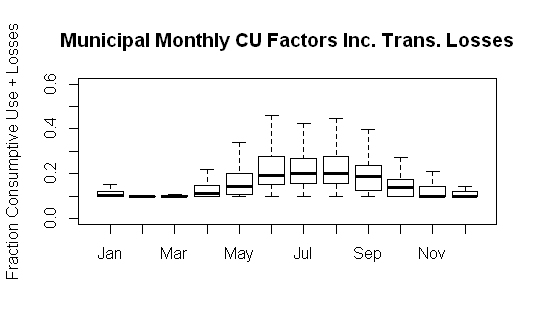
\includegraphics[scale=1.0]{sections/Xfigures/cu_wbr_unacc.png}
\caption{Summary of estimated consumptive use fractions for all municipal facilities where the Winter Base Rate method could be applied.  Median values ranged from 0.1 (10\%) to 0.2 (20\%) in the summer, with summer-time evaporative losses as high as 0.4 (40\%) in some areas.}
\end{figure}


\begin{multicols}{2}
\paragraph{Transmission Losses}\mbox{}\smallskip 
\label{sec:cu_tloss}

\noindent Municipal water systems deliver water to service areas through a large network of pipes (the distribution system) of varying age and condition, and then water is returned through another network of conveyances to the wastewater treatment facilities (the collection system).  Consequently there can be a wide range of transmissions losses, or ``leakage from pipes during water transmission".  Transmission losses may be permanently lost via evapotranspiration, they may return to the stream as base flow, or they may be delayed and effectively lost from the short term water budget.  However, estimating the amount that is permanently lost is very difficult, and can vary seasonally and annually within the same system. This model used a value of 10\% to represent the percent of water withdrawn and not returned to the stream due to transmission losses for all systems.  Improved quantification of the fate and magnitude of transmission losses in water-stressed watersheds should be prioritized in future planning efforts (more on this can be found in Appendix \ref{Appendix B}).

\end{multicols}